\documentclass[PhD-Yoann-Dupont.tex]{subfiles}
\begin{document}

CasEN \citep{nouvel2010reconnaissance} est un reconnaisseur d'entités nommées par cascade de transducteurs se basant sur la plateforme UNITEX \cite{paumier2011unitex}, développé par le Laboratoire de l'Université de Tours\footnote{\url{http://li.univ-tours.fr}}. Il a été créé dans le cadre des projets ANR Variling, FEDER Région Centre Entités nommées et nommables, Ortolang et Istex.

Le principe général de CasEn est d'utiliser à la fois des ressources externes comme des dictionnaires ainsi que des règles contextuelles pour enrichir progressivement le texte donné en entrée. Ces enrichissements donnent une sortie qui peut alors être utilisée par un autre transducteur, donnant une annotation de plus haut niveau. Par exemple, pour reconnaître une personne, un premier transducteur pourrait appliquer divers dictionnaires comme un dictionnaire de titres de civilité, un de prénoms et un de noms de famille. Ces informations peuvent alors être utilisées par un transducteur spécifique qui aurait la règle suivante: \emph{titre} \emph{prénom} \emph{nom} $\implies$ \emph{personne}. Un exemple de transducteur est donné dans la figure\ \ref{fig:casen-longueur}.

\begin{figure}[ht!]
    \centering
    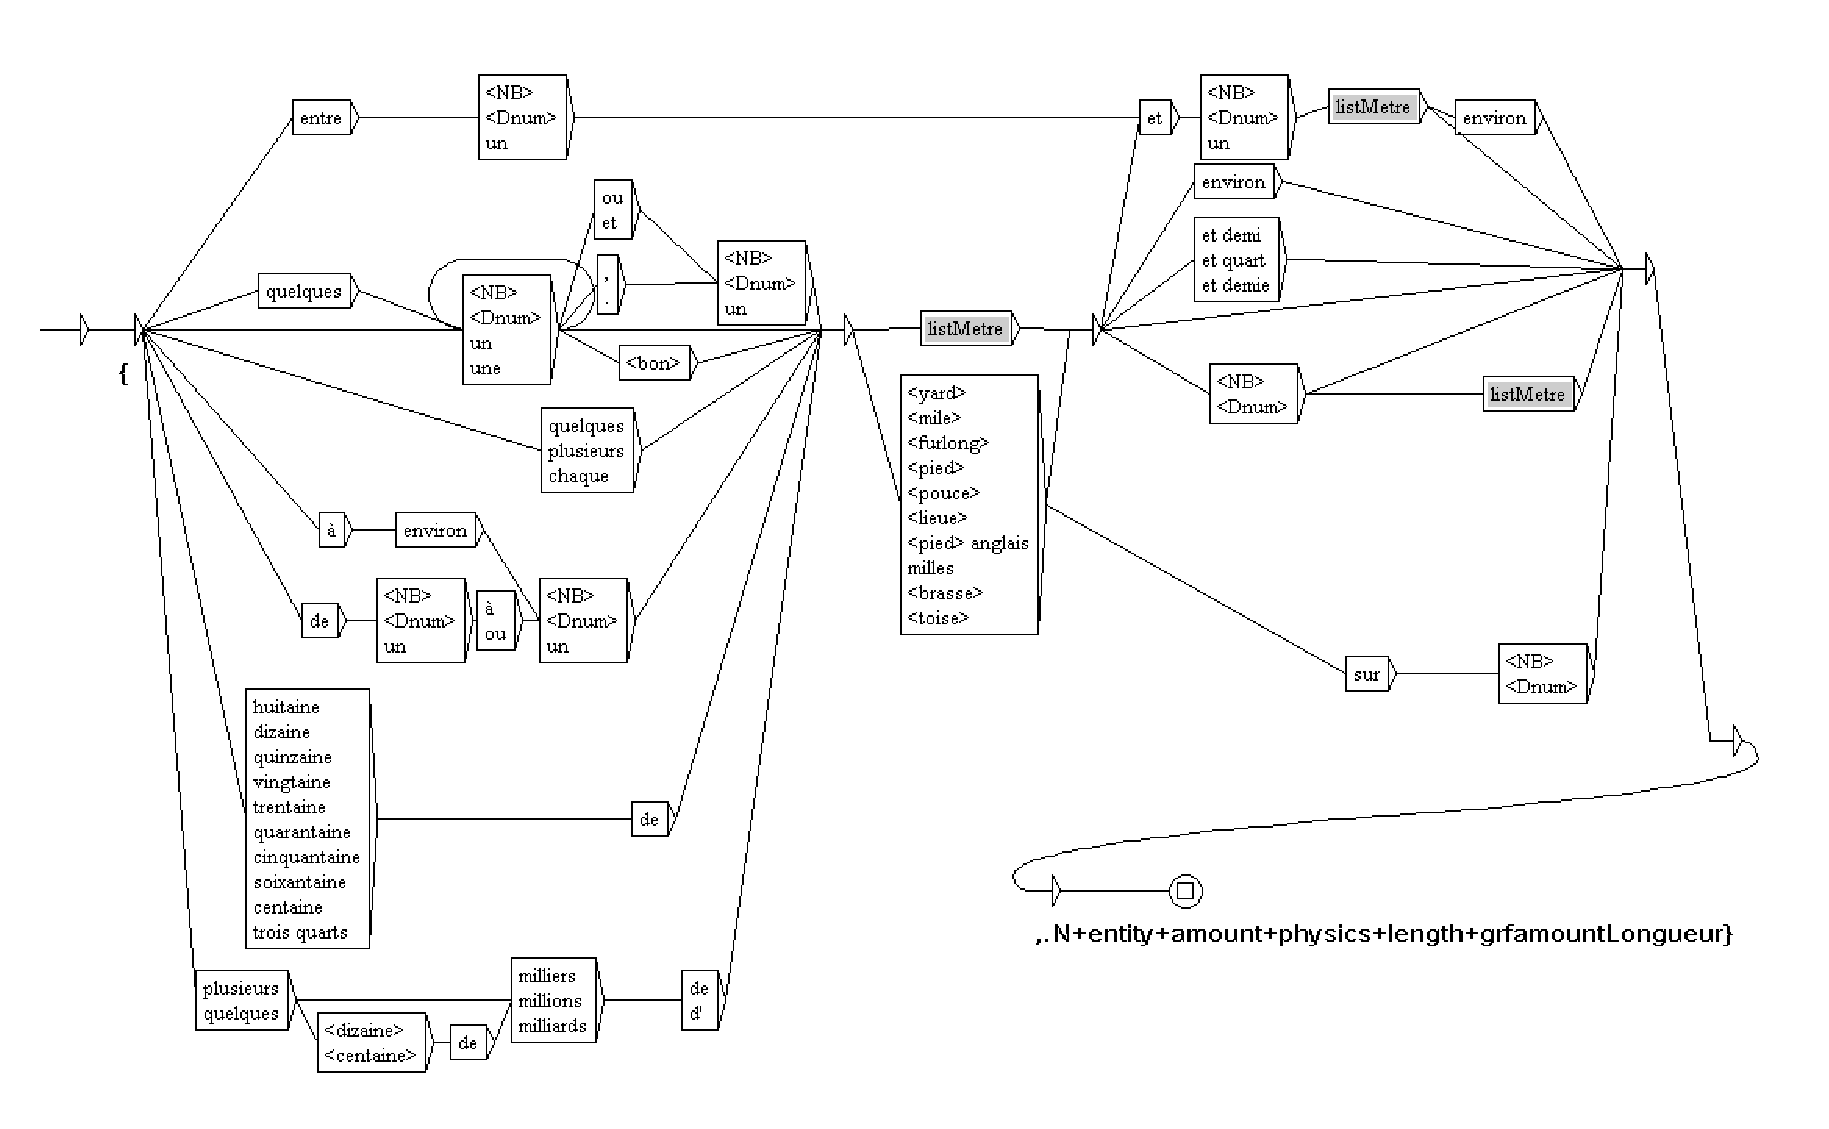
\includegraphics[scale=0.5]{images/CasEN/longueurs}
    \caption{Un automate pour traiter les longueurs}
    \label{fig:casen-longueur}
\end{figure}

\end{document}